\chapter{基于作业运行时信息及拓扑结构的缓存替换策略}\label{chap:guide}
\section{Spark系统缓存替换策略分析}

在第二章已经详细分析过Spark默认的LRU缓存替换策略。是通过BlockManager管理RDD缓存数据、Shuffle数据、BroadCast缓存数据。本章重点关注RDD缓存数据。BlockManager内部有MemoryStore和DiskStore。分别用来管理内存缓存数据以及磁盘缓存数据。MemoryStore内部是通过LinkedHashMap存储block数据,LinkedHashMap是具有LRU特性的。

Spark框架使用简单的LRU缓存替换策略是有潜在的问题的。因为LRU策略仅仅考虑了数据访问的时间特性,在缓存空间不足的时候优先替换最长时间为访问的数据。这种方法它的优点是实现方法简单,时间复杂度低,在CPU Cache缓存场景是很合适的,因为Cache中数据大小一样,内存访问请求对与CPU来说也具有相同的重要性,因为从CPU的视角来看,不同的物理地址并没有什么不同。另一个方面,LRU缓存策略比较简单,在CPU物理器件内部比较容易实现。所以在CPU缓存场景下,LRU这种缓存替换策略是很适用的。但是对于Spark框架来说,LRU策略就有一些不足。因为不同的RDD具有不同的重要性,数据大小也不同。有的RDD数据是通过复杂计算,耗费了很长时间计算得到的。并且对于整个DAG计算图来说,不同的RDD的重要性也各不相同。如果对DAG中的关键路径的RDD节点,如果发生了数据丢失就会影响到整个DAG计算图作业的端到端执行时间。所以对LRU缓存替换策略进行进一步的改进,对于提升任务执行效率,减少任务端到端执行时间具有重要的意义。

\section{基于作业运行时信息及拓扑结构的缓存替换策略的设计与实现}

\subsection{替换替换策略设计}

本文提出了一种基于DAG作业运行时信息以及DAG计算图拓扑结构的缓存替换策略。缓存管理模块会实时采集作业执行中的信息,比如作业执行时间,数据大小。并且根据DAG计算图的拓扑结构动态调整缓存优先级,提高缓存数据是使用效率并减少作业端到端执行时间。详细的说,本文提出了一种缓存数据优先级计算算法。该算法综合考虑DAG图中前驱作业执行状况,DAG图拓扑关系动态计算各个缓存数据的优先级。通过将重要数据的优先级变高,从而保证发生缓存数据替换的时候能够将从整个DAG时间来看优先级较低的数据替换删除,这样就可以将重要数据一直保存在内存缓存之中,这样在之后的作业执行过程中缓存数据就有更高的使用效率,从而可以提高整体作业的执行效率。

\subsubsection{RDD访问次数}

Spark应用在计算过程中,为了加快计算过程,会将重复使用的RDD数据缓存在内存之中,在计算过程中通过重复访问内存中的RDD数据达到计算计算过程的功能。所以可见,RDD数据的访问次数是一个很关键的指标,重复访问次数多的数据应该加大优先级,优先保存在缓存之中。

对于RDD的复用次数可以通过分析DAG图结构得到,如图\ref{fig:spark-dag}所示,可以看到RDD1有两个出度,所以RDD1数据就会被使用到两次,会计算得到RDD2和RDD3。而图中其他RDD数据的出度都为1,所以其他数据都不会被复用。可见可以通过RDD节点的出度判断重复使用的次数。$RDD_{out}$表示RDD节点的出度,$RDD_{reuse}$表示RDD数据被重复使用的次数,$RDD_{reuse}$越大优先级就应该越高。两者的关系如公式\eqref{eq:reuse}所示。因为出度大于1说明会被重复使用,这样RDD数据才会被重复使用,所以才有放入缓存之中的价值,所以需要对出度减去一。

\begin{equation} \label{eq:reuse}
    \adddotsbeforeeqnnum%
    RDD_{reuse} = RDD_{out} - 1
\end{equation}

\begin{figure}[htbp]
    \centering
    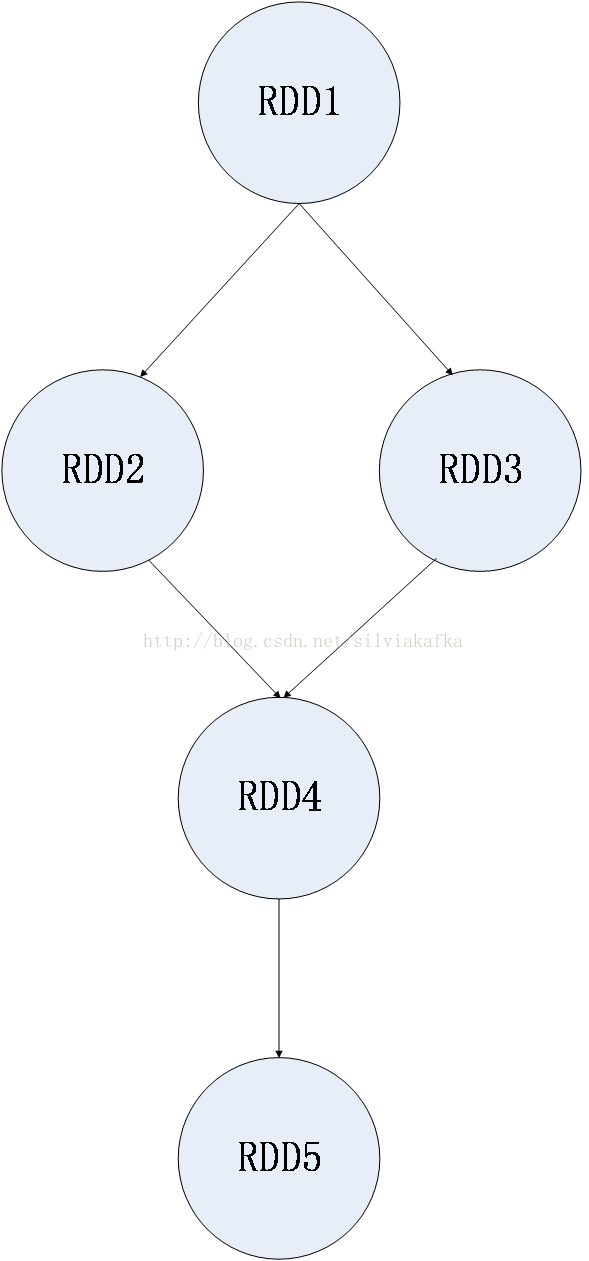
\includegraphics[width=0.4\textwidth]{Img/spark-dag.png}
    \caption{Spark DAG示意图}
    \label{fig:spark-dag}
\end{figure}

\subsubsection{RDD数据大小}

通过对Spark缓存管理原理分析可知,Spark框架将RDD数据分为多个partition分区,分区分布在不同的Executor之中。所有partition的位置通过blockManager同意管理。Spark框架将Executor申请的内存分为多个区域,需要用于框架执行,用户代码执行,数据缓存等多种用途,实际用于数据缓存的内存空间是非常优先的,所以为了提高内存空间的使用效率,在其他因素相同的情况下,应该优先缓存数据量比较小的RDD数据,这样就可以有效节省内存空间。这里将RDD数据大小记为$RDD_s$。

\subsubsection{RDD计算代价}

在一个DAG图中,每个节点都是RDD数据,节点之间的边都为RDD之间的转化关系,为transform和action两种之一的算子,而不同的算子操作的计算代价是非常大的。比如对于$map,filter$等操作原理相对比较简单,这类算子的底层原理是对每个partion进行同样的操作处理,但是用户可以自定义操作函数,用户自定义的操作处理可能会非常复杂。而join算则的实现原理就非常复杂,框架需要根据数据大小决定使用BroadcastJoin或是sort merge join。上文已经介绍过两种join操作的实现原理,sort merge join尤其比较复杂,参与join操作的表首先需要通过shuffle将相同key的数据发送到同一个分区,shuffle操作也可以保证数据是排序的,然后通过类似merge sort的原理将两个表合并在一起。

通过分析可以看到,不同的算子操作的时间复杂度是非常难以预料的,所以也应该将数据分区的计算代价当作重要考虑因素。对于计算代价非常高的RDD数据来说就应该将其优先存储在缓存之中,因为如果计算代价高的RDD数据一旦丢失,就需要重新计算,就会造成巨大的重复计算开销。

如果$RDD_i$通过转化操作得到$RDD_j$,那么就说$RDD_i$是$RDD_j$的父节点。将$C_{ij}$记为i,j数据之间转化操作的开销。通过这种方式DAG图中的每天边都有了全职,成为了带权的DAG图。

\subsubsection{根据DAG拓扑结构计算RDD优先级}

Spark应用程序会组成一个DAG计算图。DAG图中的节点为RDD数据,DAG图中的边为RDD之间的转换关系。不同的点也就是RDD数据大小各不相同,不同的边也就是RDD之间的转换关系的计算代价也各不相同。所以Spark应用的执行过程可以看作是对DAG图的遍历过程,端到端的执行时间为输入节点到输出节点的最短路径中最短的一条路径。这一条路径也就是DAG图的关键路径。所以缓存替换策略应该考虑整体DAG图的拓扑结构。对于关键路径中的RDD缓存数据应该尽量保存在缓存之中,应为如果将关键路径中的RDD数据替换出去,在之后的计算过程中如果访问到替换出去的数据,发现数据丢失,框架就就根据容错原理,根据拓扑结构重复计算丢失的数据,这样就会极大地增加端到端的执行时间。

\subsection{缓存替换策略实现}

综上所述应该综合考虑数据大小,复用次数,计算代价等因素计算RDD节点的优先级。Spark会将应用程序转化为一个DAG图,这里使用$G(V, E)$来表示DAG。DAG图中的节点$V$是RDD数据,DAG图中的边$E$为RDD数据之间的转化关系。如果$RDD_i$通过操作转化为$RDD_j$,其中存在一条边$(i, j)\in E$,那么$RDD_i$就称为$RDD_j$的父节点。对于$RDD_v$来说,它的所有父节点记为$anc(v)$。它的所有后继节点记为$dsc(v)$。边$(i,j)$的权重$C_{ij}$为计算开销。然后可以通过算法\ref{alg:rdd-cost}计算得到当前RDD节点的重复计算代价。$C_{ij}$要在计算过程中实时更新,每次执行完一个操作之后就更新DAG图中的边的权值,然后通过算法计算RDD的重复计算代价。这里通过$RDD_{cost}$记录RDD数据的重复计算代价。

\begin{algorithm}  
    \caption{计算RDD的重复计算代价}  
    \begin{algorithmic}[1] %每行显示行号  
        \Require DAG图根节点
        \Ensure 所有RDD的重复计算代价
        \Function{CALCULATE\_ALL\_COST}{$RDD \ root, \ HashMap \ cost$}
            \State $ancestors \gets root.getAncestors()$
            \State $curId \gets root.getId()$
            \State $edgeCost \gets 0$
            \For{$ancestor \in ancestors$}
                \State $preId \gets ancestor.getId()$
                \State $edges \gets root.getInEdges()$
                \State $edge \gets null$
                \For{$e \in edges$}
                    \If{$e.getStart() == preId$}
                        \State $edge \gets e$
                    \EndIf
                \EndFor
                \State $edgeCost = max(edgeCost, \ edge.getCost)$
            \EndFor
            \State $cost[root] \gets edgeCost$
            \State $successors \gets root.getSuccessors()$
            \For{$successor \in successors$}
                \State \Call{$CALCULATE\_ALL\_COST$}{$successor, \ cost$}
            \EndFor
        \EndFunction
    \end{algorithmic}
    \label{alg:rdd-cost}
\end{algorithm}

本文通过几个因素综合计算RDD权重。包括RDD重复计算代价$RDD_{cost}$,分区大小$RDD_s$,RDD的重复使用次数$RDD_{reuse}$,来计算RDD的缓存优先级$RDD_{weight}$。

\begin{equation} \label{eq:weight}
    \adddotsbeforeeqnnum%
    RDD_{weight}=a \times RDD_{reuse} + b \times RDD_{cost} - c \times RDD_{s}
\end{equation}

其中a,b,c分别对应RDD重复使用次数,RDD重复计算开销,RDD大小的权重系数。应该都是大于等于0的,具体数值可以根据使用场景调整。其中重复使用次数和重复计算开销比较大的RDD数据应该优先缓存,数据规模比较大的RDD数据在同等条件下则应该替换清除,以提高内存使用效率。

\section{测试结果分析}
\section{本章总结}